\documentclass[11pt]{article}

% --- Encoding & Language ---
\usepackage[utf8]{inputenc}
\usepackage[T1]{fontenc}
\usepackage[english]{babel}

% --- Math Packages ---
\usepackage{amsmath, amssymb, amsfonts}
\usepackage{mathtools}
\usepackage{physics}          % for \dv, \pdv, \grad, etc.
\usepackage{bm}               % for bold math symbols
\usepackage{siunitx}          % for units

% --- Page Layout ---
\usepackage[margin=1in]{geometry}
\usepackage{setspace}
\onehalfspacing

% --- Theorem Environment ---
\usepackage{amsthm}
% Create a shared counter (let's call it 'statement') per section
\newtheorem{statement}{Statement}[section]
\newtheorem{theorem}[statement]{Theorem}
 
% Define 'assumption' and 'diagram' to use the same counter
\newtheorem{assumption}[statement]{Assumption}
\newtheorem{diagram}[statement]{Diagram}
\newtheorem{note}[statement]{Note}

% --- Figure & Table ---
\usepackage{graphicx}
\usepackage{float}
\usepackage{caption}
\usepackage{subcaption}
\usepackage{mwe}
% \includegraphics{example-image}
\usepackage{hyperref}

% --- TikZ for Diagrams ---
\usepackage{tikz}
\usetikzlibrary{arrows.meta, decorations.pathmorphing, patterns}

% --- Code Listings (optional) ---
\usepackage{listings}
\lstset{
  basicstyle=\ttfamily\small,
  frame=single,
  breaklines=true,
  postbreak=\mbox{\textcolor{red}{$\hookrightarrow$}\space},
}


% --- Title Info ---
\title{\textbf{Force Based Model Analysis}}
\author{Jerry Wu}
\date{\today}

\begin{document}

\maketitle
\noindent
\textbf{Helpful Link:}
\begin{itemize}
    \item \href{https://www.geogebra.org/classic/vzgc97bq}{Geogebra Demo}
    \item \href{https://www.canva.com/design/DAGo-OCr6Yo/K5YV57vaBxux-PqkqwI4ow/edit?utm_content=DAGo-OCr6Yo&utm_campaign=designshare&utm_medium=link2&utm_source=sharebutton}{Canva Graphics}
\end{itemize}

% \begin{assumption}\label{ass:leg-ground-contact}
% The end point of each leg is always contacting the ground.
% \end{assumption}

\begin{assumption}\label{ass: no-body-contact}
The robot body would never contact with the terrain
\end{assumption}

\begin{assumption}\label{ass: com}
The CoM of the robot is always at local geometric center in direction parrallel to Spine
\end{assumption}

\section{Statics}
\begin{assumption}
Static means the robot would not move and achieve static equilibrium in this state
\end{assumption}
\subsection*{Slope}

\begin{diagram}
    Simple case where two legs have same height
\end{diagram}\label{ass:h2-equal-h1}
\vspace{1ex} % small vertical space
\begin{center}
    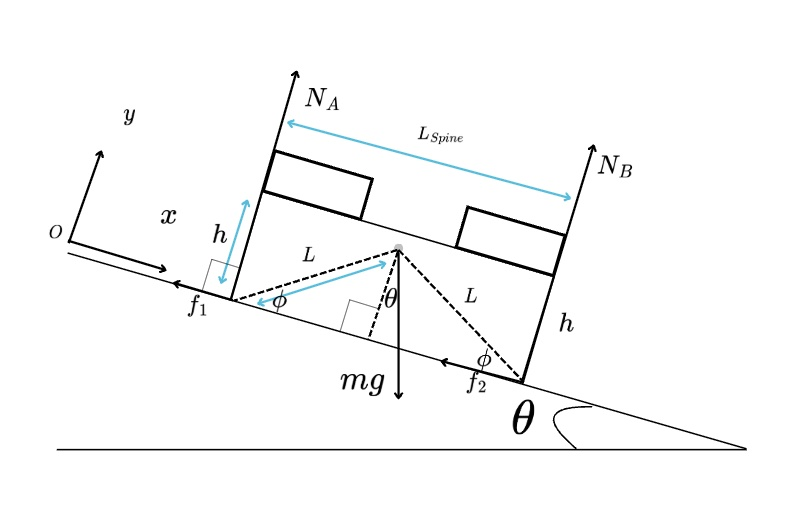
\includegraphics[width=0.6\textwidth]{figs/Simple case where two legs have same height.jpg} % replace with your image
\end{center}

To start with,  we put robot on a slope with angle \(\theta\). To make the analysis easier,
assume that two leg have same height \(h\) in this case. Therefore, the moment arm are symetric
for \(R_A\) and \(R_B\). Therefore, we can get follow equations:
\[ \sum F_x = (f_1+f_2) - \sin(\theta)mg = 0 \]
\[ \sum F_y = (N_A+N_B) - \cos(\theta)mg = 0 \]
\[ \sum M_A = L_\text{spine} \cdot N_B -  L \cdot mg \cdot \sin(\frac{\pi}{2}-\phi+\theta) = 0 \]
\[ \sum M_B = L_\text{spine} \cdot N_A -  L \cdot mg \cdot \sin(\frac{\pi}{2}-\phi+\theta) = 0 \]

\begin{diagram}
    Two legs have different height
\end{diagram}\label{ass:h2-larger-than-h1}
\vspace{1ex} % small vertical space
\begin{center}
    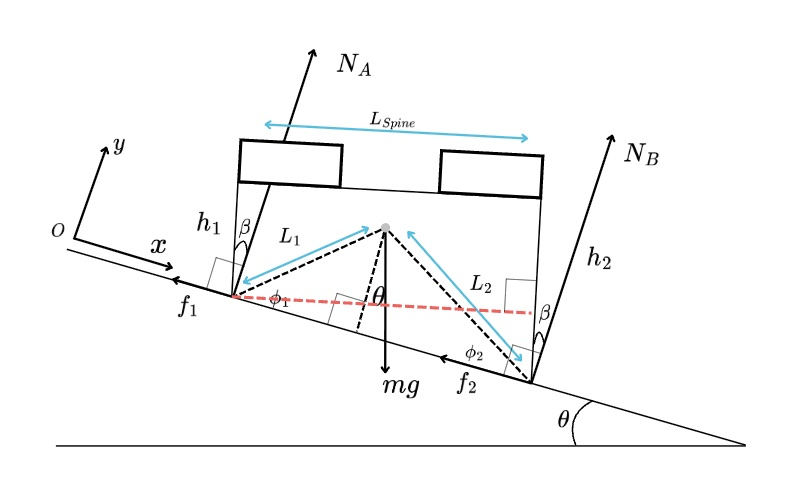
\includegraphics[width=0.5\textwidth]{figs/Two legs have different height.jpg} % replace with your image
\end{center}

Now extend the case to where the leg length would change. Here the robot extended
the right leg to \(h_2\), which makes the robot rotate angle \(\beta\) around
the z-Axis. Now both moment arms on two legs are 
shifted. We can also form the static equilibrium equation as follows:

\[ \sum F_x = (f_1+f_2) - \sin(\theta)mg = 0 \]
\[ \sum F_y = (N_A+N_B) - \cos(\theta)mg = 0 \]
\[ \sum M_A = \frac{L_\text{spine}}{\sin(\frac{\pi}{2}-\beta)} \cdot N_B \cdot \sin(\frac{\pi}{2})-  L_1 \cdot mg \cdot \sin(\frac{\pi}{2}-\phi_1+\theta) = 0 \]
\[ \sum M_B = \frac{L_\text{spine}}{\sin(\frac{\pi}{2}-\beta)} \cdot N_A \cdot \sin(\frac{\pi}{2})-  L_2 \cdot mg \cdot \sin(\frac{\pi}{2}-\phi_2-\theta) = 0 \]

based on the geometry of our robot, we can also formulate:
\[L_\text{spine} \cdot \cos(\frac{\pi}{2}-\beta) = h_2 - h_1 \]

\begin{note}\label{not:what-is-known}
\(h_1\), \(h_2\) are known values, so \(\beta\) is also known.  
Therefore, \(\phi_1\) and \(\phi_2\) can easily be solved using Theorem~\ref{thm:law-of-cosines}.
\end{note}

\begin{theorem}\label{thm:law-of-cosines}
Law of Cosines

\[
\cos A = \frac{b^2 + c^2 - a^2}{2bc}
\]
\[
\cos B = \frac{a^2 + c^2 - b^2}{2ac}
\]
\[
\cos C = \frac{a^2 + b^2 - c^2}{2ab}
\]
\end{theorem}


\subsection*{Zig-Zag Terrain}

\begin{assumption}\label{ass:Zig-Zag-terrain-assumption}
The terrain is uniform that all triangle obstable and gap between them are same
\end{assumption}

A natural extension for the slope is triangle terrain. There are esseintially five cases
when robot is static on the triangle terrain: 1. two legs on the same slope 2. two legs on two slopes that face each other
3. two legs on two slopes that does not face each other 4. one leg is on the slope and the other is on the gap. 5. two legs
are all on the gap. 

For case 1, we have already discussed in the previous section. And for case 5, it is esseintially the same
like slope when \(\theta\) is 0.

\begin{diagram}
    Case2: two legs on the slope that face each other
\end{diagram}
\vspace{1ex} % small vertical space
\begin{center}
    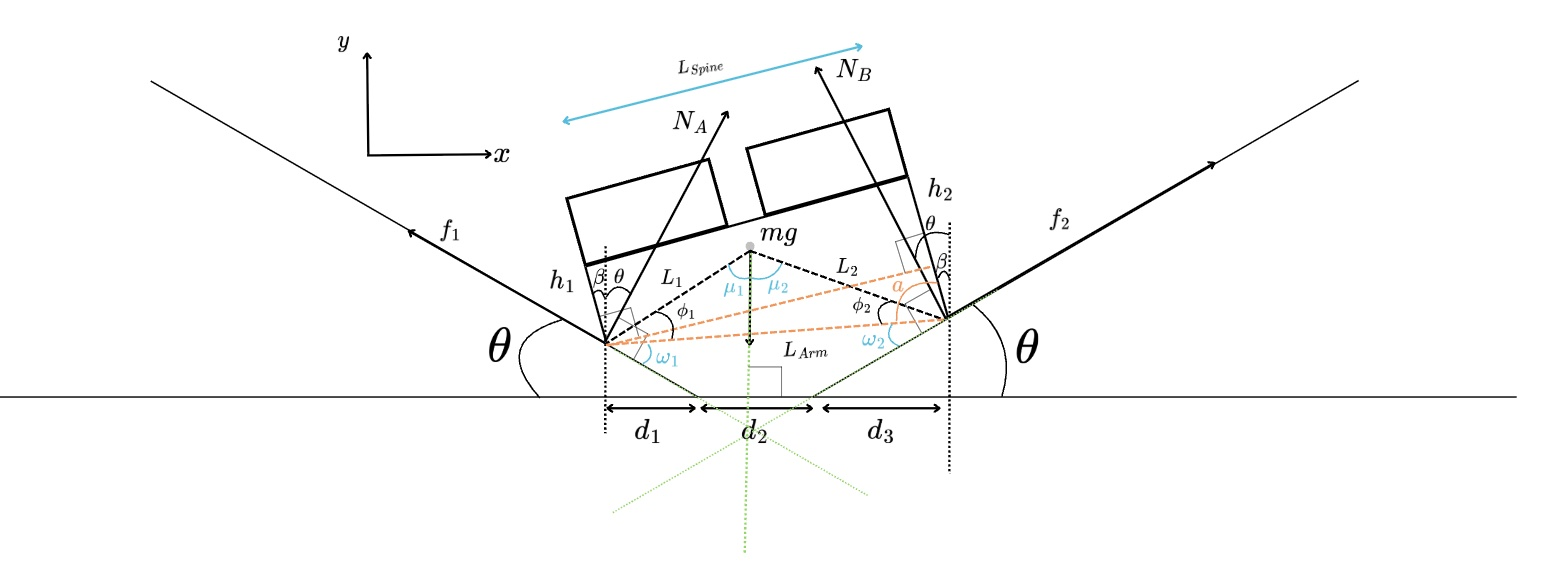
\includegraphics[width=0.7\textwidth]{figs/Case2.jpg} % replace with your image
\end{center}

To make it clearer, I changed the coordinate that aligns with the ground rather slope from now on.
We can also formulate the equilibrium equations:

\[ \sum F_x = (-f_1+f_2)\cos(\theta) + (N_A-N_B) \sin(\theta) = 0 \]
\[ \sum F_y = (f_1+f_2)\sin(\theta) + (N_A+N_B) \cos(\theta) - mg = 0 \]
\[ \sum M_A =  L_\text{Arm} \cdot (N_B \cdot \sin(\frac{\pi}{2}-\omega_2) + f_2 \cdot \sin(\pi-\omega_2)) - L_1\cdot mg \cdot \sin(\mu_1)= 0 \]
\[ \sum M_B =  L_\text{Arm} \cdot (N_B \cdot \sin(\frac{\pi}{2}-\omega_1) + f_1 \cdot \sin(\pi-\omega_1)) - L_2\cdot mg \cdot \sin(\mu_2)= 0 \]

where by geometry of the shape, we can find:
\[\omega_1 = (\theta + \beta)  - (\frac{\pi}{2}-\alpha) \]
\[\omega_2 = (\theta - \beta) + (\frac{\pi}{2}-\alpha) \]
\[\mu_1 = \pi-(\phi_1+\omega_1)-(\frac{\pi}{2}-\theta) \]
\[\mu_2 = \pi-(\phi_2+\omega_2)-(\frac{\pi}{2}-\theta) \]
\[\alpha = \arctan(\frac{L_\text{Spine}}{h2-h1}) \]
\[L_\text{Arm} = \sin(\alpha) \cdot L_\text{Spine}\]

similarly to Note~\ref{not:what-is-known}, this equalion can be solved.

\begin{diagram}
    Case3: two legs on two slopes that do not face each other
\end{diagram}
\vspace{1ex} % small vertical space
\begin{center}
    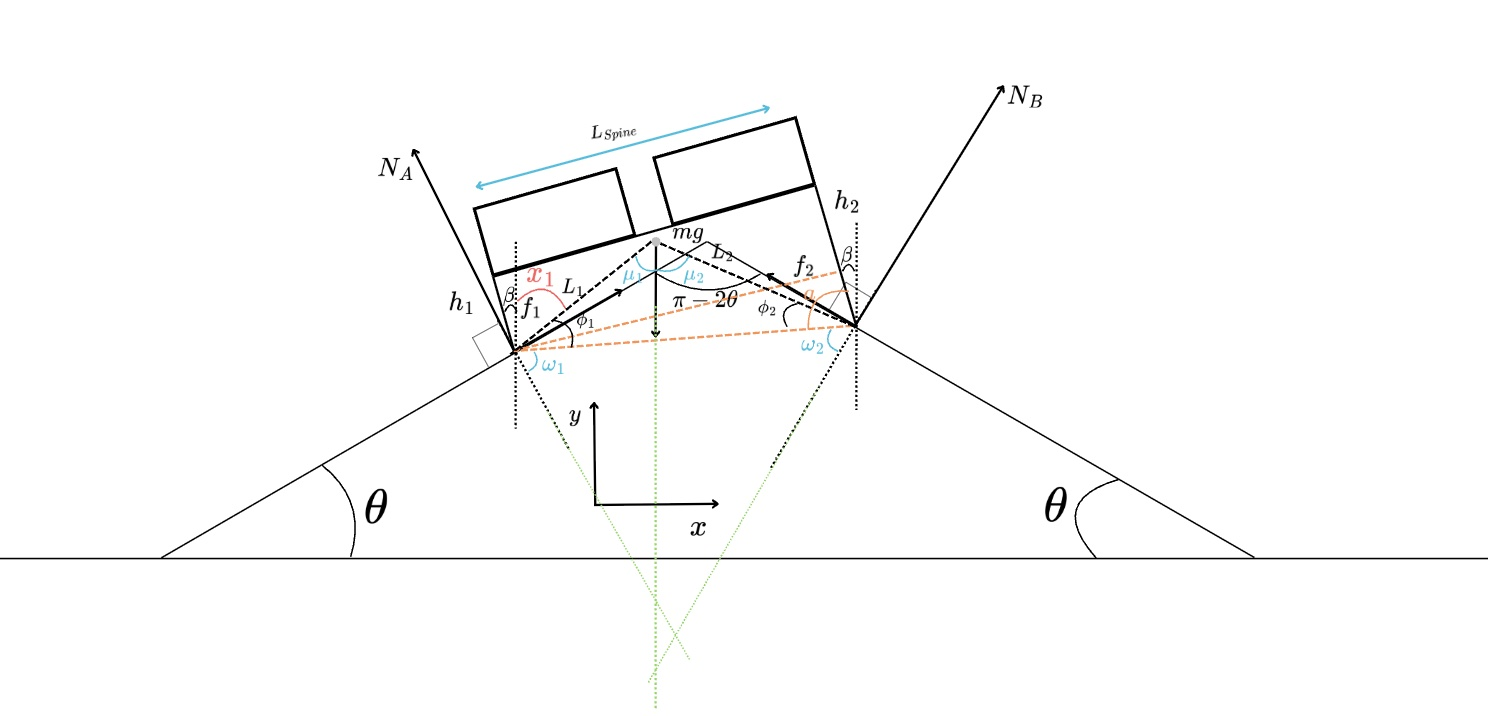
\includegraphics[width=0.7\textwidth]{figs/Case3.jpg} % replace with your image
\end{center}

\[ \sum F_x = (f_1-f_2)\cos(\theta) + (-N_A+N_B) \sin(\theta) = 0 \]
\[ \sum F_y = (f_1-f_2)\sin(\theta) + (-N_A+N_B) \cos(\theta) - mg = 0 \]
\[ \sum M_A =  L_\text{Arm} \cdot (N_B \cdot \sin(\pi-\omega_2) + f_2 \cdot \sin(\frac{\pi}{2}-\omega_2)) - L_1\cdot mg \cdot \sin(\mu_1)= 0 \]
\[ \sum M_B =  L_\text{Arm} \cdot (N_A \cdot \sin(\pi-\omega_1) + f_1 \cdot \sin(\frac{\pi}{2}-\omega_1)) - L_2\cdot mg \cdot \sin(\mu_2)= 0 \]

where by geometry of the shape, we can find:
\[\omega_1 = \beta + \alpha - \theta\]
\[\omega_2 =  \pi - \beta - \alpha - \theta\]
\[\mu_1 = \pi-(\phi_1+\omega_1)-\theta \]
\[\mu_2 = \pi-(\phi_2+\omega_2)-\theta \]
\[\alpha = \arctan(\frac{L_\text{Spine}}{h2-h1}) \]
\[L_\text{Arm} = \sin(\alpha) \cdot L_\text{Spine}\]

\begin{note}
The equation for \(\omega_1\)  can be found specifically by following equation:
\end{note}
\begin{equation}
x_1 + \phi_1 + \omega_1 + \theta = \pi
\end{equation}

\begin{equation}
\beta + x_1 + \phi_1 - \left( \frac{\pi}{2} - \alpha \right) = \frac{\pi}{2}
\end{equation}

\begin{equation}
\omega_1 = \beta + \alpha - \theta
\tag*{From (1) and (2)}
\end{equation}

\begin{diagram}
    Case4: one leg is on the slope and the other is on the gap
\end{diagram}
\vspace{1ex} % small vertical space
\begin{center}
    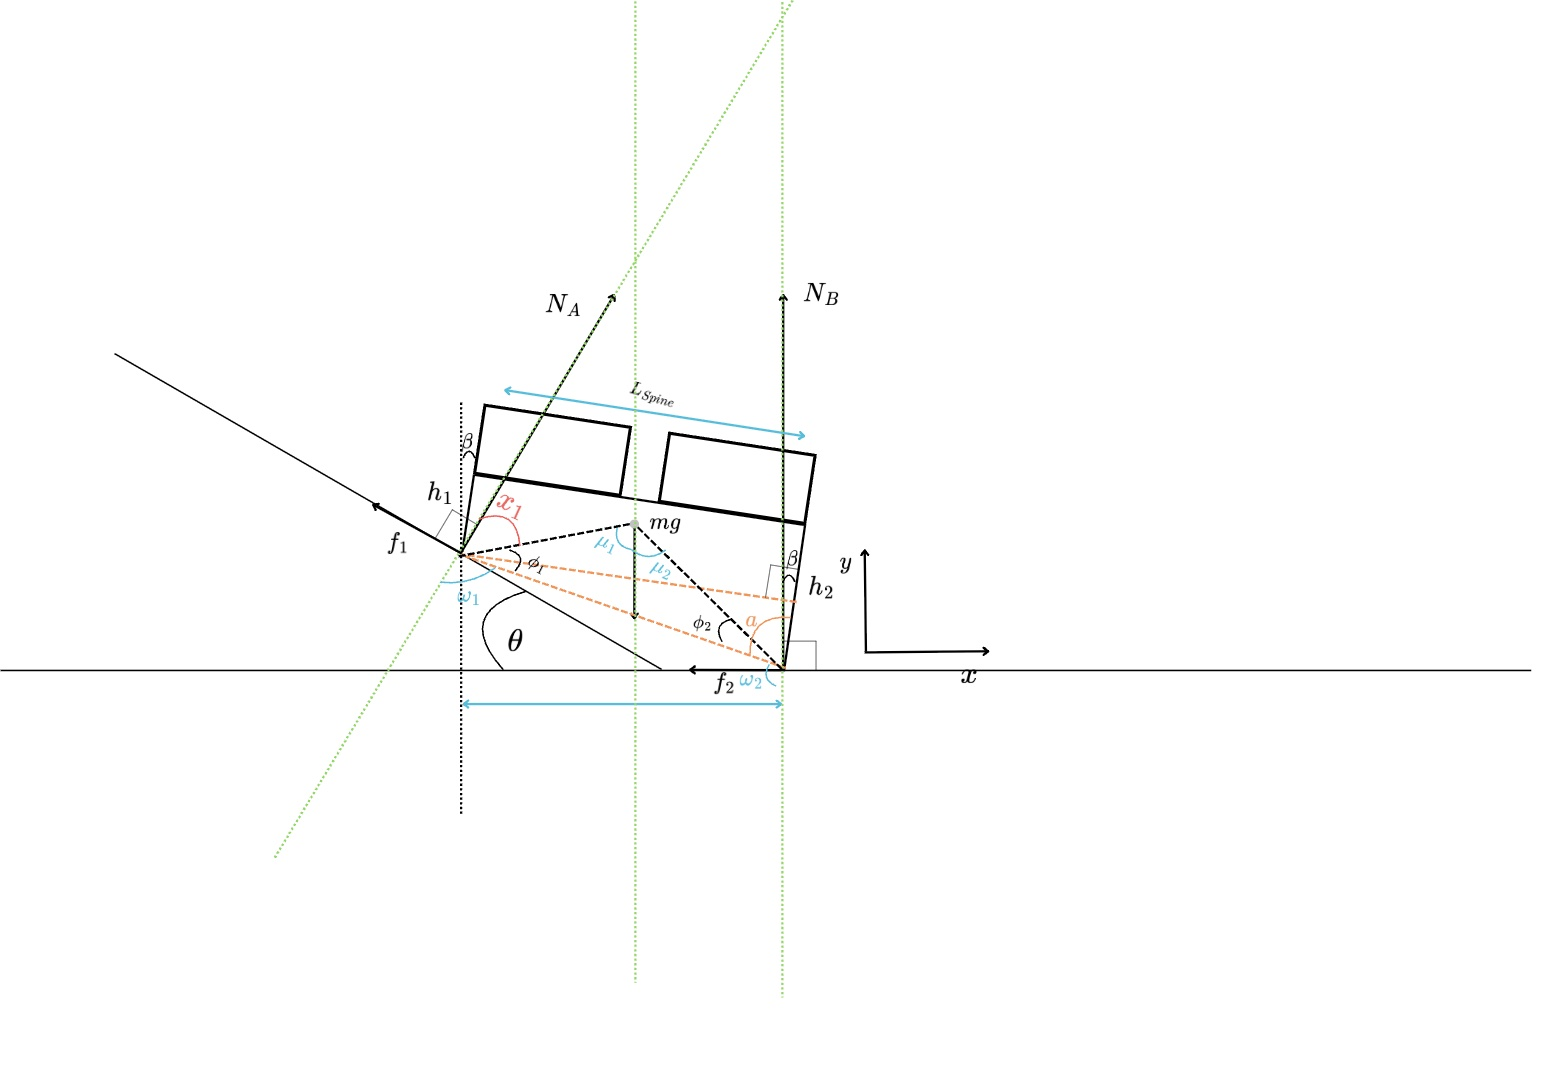
\includegraphics[width=0.7\textwidth]{figs/Case4.jpg} % replace with your image
\end{center}

\[ \sum F_x = -f_1 \cos(\theta) -f_2 + N_A \sin(\theta)= 0 \]
\[ \sum F_y = f_1 \sin(\theta)+ N_A \cos(\theta) + N_B - mg = 0 \]
\[ \sum M_A =  L_\text{Arm} \cdot (N_B \cdot \sin(\pi-\omega_2) + f_2 \cdot \sin(\frac{\pi}{2}-\omega_2)) - L_1\cdot mg \cdot \sin(\mu_1)= 0 \]
\[ \sum M_B =  L_\text{Arm} \cdot (N_B \cdot \sin(\pi-\omega_1) + f_1 \cdot \sin(\frac{3\pi}{2}-\omega_1)) - L_2\cdot mg \cdot \sin(\mu_2)= 0 \]

where by geometry of the shape, we can find:
\[\omega_1 = \theta - \beta + \alpha\]
\[\omega_2 =  \pi + \beta - \alpha \]
\[\mu_1 = \pi-(\phi_1+\omega_1)-\theta \]
\[\mu_2 = \pi-(\phi_2+\omega_2) \]
\[\alpha = \arctan(\frac{L_\text{Spine}}{h2-h1}) \]
\[L_\text{Arm} = \sin(\alpha) \cdot L_\text{Spine}\]

\begin{note}
The equation for \(\omega_1\)  can be found specifically by following equation:
\end{note}
\begin{equation}
x_1 + \phi_1 + \omega_1 = \pi
\end{equation}

\begin{equation}
\theta-\beta + x_1 + \phi_1 - \left( \frac{\pi}{2} - \alpha \right) = \frac{\pi}{2}
\end{equation}

\begin{equation}
\omega_1 = \theta - \beta + \alpha
\tag*{From (1) and (2)}
\end{equation}

Now, by observation, this case is very similar to previous case. In fact, all of the above cases
are geometrically similar, which means we can find a general expression for this force based model.

\begin{diagram}
    Determine the geometry shape by robot body and terrain
\end{diagram}
\vspace{1ex} % small vertical space
\begin{center}
    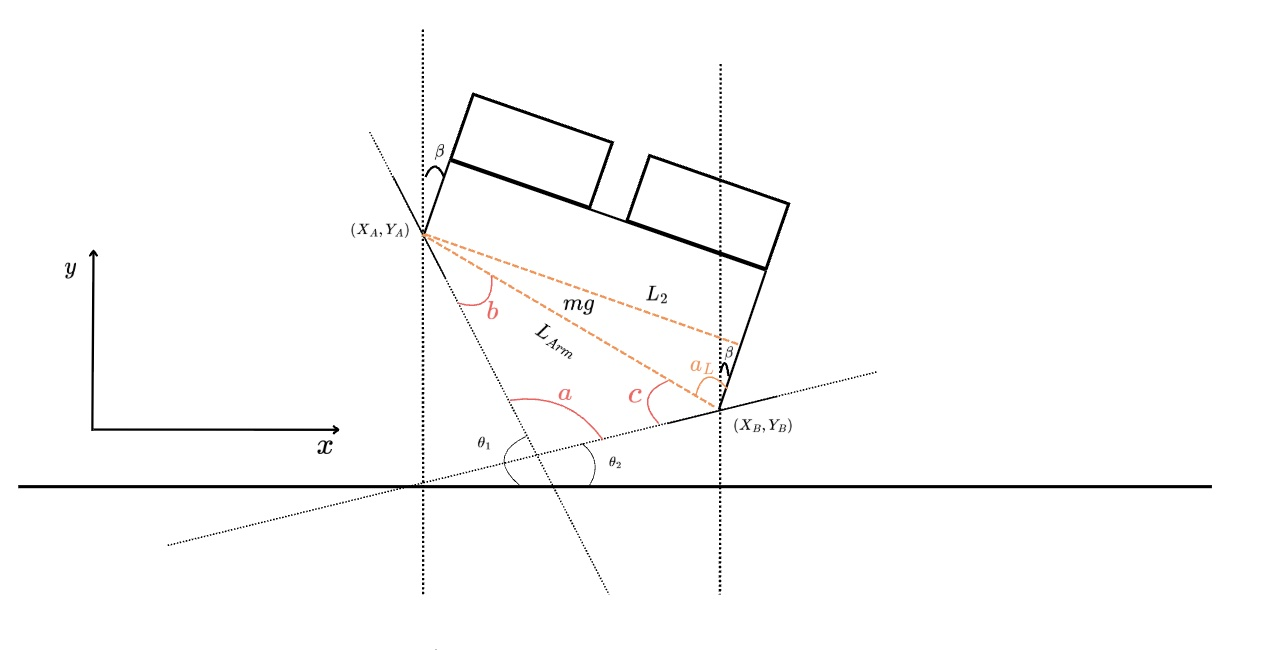
\includegraphics[width=0.5\textwidth]{figs/geometry shape.jpg} % replace with your image
\end{center}

After simplifying the model, it can be seen that given the terrain tangent angle \(\theta_1\), \(\theta_2\), robot pitch
angle \(\beta\) and length of the virtual link between end point of two leg \(L_{Arm}\) we can determine the triangle with
inner angle \(a,b,c\). 

Here is how we determine angle \(a, b, c\):
\[a = \pi - \theta_1 - \theta_2\]
\[b = \pi - \beta - \frac{\pi}{2}-(\frac{\pi}{2}-\alpha_L)-(\pi-\theta_1)\]
\[c = \pi - (\pi-\theta_2) + \beta - \alpha_L\]

by verification: 
\[a+b+c = \pi\]

As for different tangent angles, this property should hold as well. This means there would be \textbf{only one solution} by
given condition.

\begin{diagram}
    Generailized Free Body Diagram
\end{diagram}
\vspace{1ex} % small vertical space
\begin{center}
    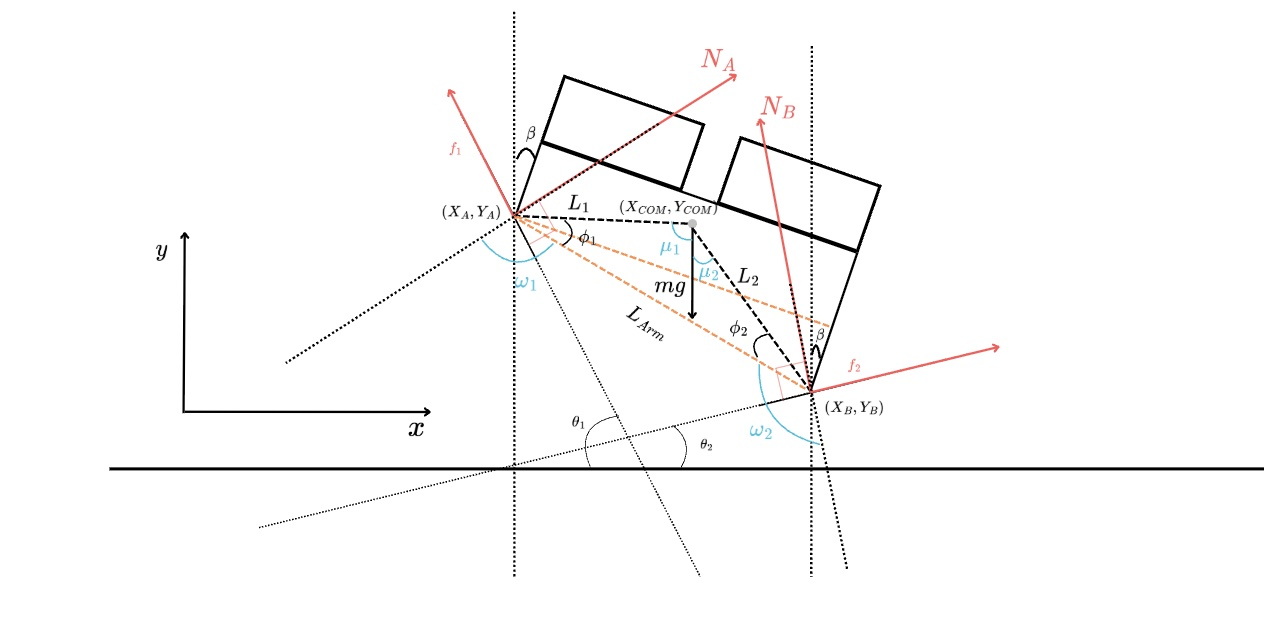
\includegraphics[width=0.8\textwidth]{figs/Generailized.jpg} % replace with your image
\end{center}

Given the determined geometric shape of the robot and terrain, we can easily find the position of the COM through
the given of relative position \(L_1\) and \(L_2\), which can be solved by the geometry as well. Which means, if we put
the robot into coordinate, the points \((X_A, Y_A), (X_B, Y_B), (X_{COM}, Y_{COM})\) are given.


Therefore, given \((X_A, Y_A), (X_B, Y_B), (X_{COM}, Y_{COM}), \theta_1, \theta_2\), \(L_{Spine}\) we can formulate
\[
\sum \vec{F} = \vec{f}_1 + \vec{f}_2 + \vec{N}_A + \vec{N}_B + \vec{W} = \vec{0}
\]

\[
\sum \vec{M}_A = 
(\vec{r}_B - \vec{r}_A) \times (\vec{f}_2 + \vec{N}_B)
+ (\vec{r}_{\text{COM}} - \vec{r}_A) \times \vec{W}
= 0
\]

\[
\sum \vec{M}_B = 
(\vec{r}_A - \vec{r}_B) \times (\vec{f}_1 + \vec{N}_A)
+ (\vec{r}_{\text{COM}} - \vec{r}_B) \times \vec{W}
= 0
\]

where
\begin{align*}
\hat{t}_1 &= (\cos(\pi-\theta_1),\; \sin(\pi-\theta_1)) \quad \text{(contact tangent 1)} \\
\hat{n}_1 &= (-\sin(\pi-\theta_1),\; \cos(\pi-\theta_1)) \quad \text{(contact normal 1)} \\
\hat{t}_2 &= (\cos\theta_2,\; \sin\theta_2) \\
\hat{n}_2 &= (-\sin\theta_2,\; \cos\theta_2)
\end{align*}

\begin{align*}
\vec{f}_1 &= f_1 \cdot \hat{t}_1 = f_1 \cdot (\cos(\pi-\theta_1),\; \sin(\pi-\theta_1)) \\
\vec{N}_A &= N_A \cdot \hat{n}_1 = N_A \cdot (-\sin(\pi-\theta_1),\; \cos(\pi-\theta_1)) \\
\vec{f}_2 &= f_2 \cdot \hat{t}_2 = f_2 \cdot (\cos\theta_2,\; \sin\theta_2) \\
\vec{N}_B &= N_B \cdot \hat{n}_2 = N_B \cdot (-\sin\theta_2,\; \cos\theta_2) \\
\vec{W}   &= -mg \cdot (0,\; 1)
\end{align*}


\begin{align*}
\text{Moment arm of } \vec{f}_2, \vec{N}_B \text{ about A}: \quad
& \vec{r}_{f_2/A} = \vec{r}_B - \vec{r}_A = (X_B - X_A,\; Y_B - Y_A) \\
\text{Moment arm of } \vec{W} \text{ about A}: \quad
& \vec{r}_{W/A} = \vec{r}_{\text{COM}} - \vec{r}_A = (X_{COM} - X_A,\; Y_{COM} - Y_A) \\[1ex]
\text{Moment arm of } \vec{f}_1, \vec{N}_A \text{ about B}: \quad
& \vec{r}_{f_1/B} = \vec{r}_A - \vec{r}_B = (X_A - X_B,\; Y_A - Y_B) \\
\text{Moment arm of } \vec{W} \text{ about B}: \quad
& \vec{r}_{W/B} = \vec{r}_{\text{COM}} - \vec{r}_B = (X_{COM} - X_B,\; Y_{COM} - Y_B)
\end{align*}

Therefore,
\begin{align*}
    \sum \vec{F}_x &= -f_1 \cos\theta_1 + f_2 \cos\theta_2 
                     - N_A \sin\theta_1 - N_B \sin\theta_2 = 0 \\
    \sum \vec{F}_y &= f_1 \sin\theta_1 + f_2 \sin\theta_2 
                     - N_A \cos\theta_1 + N_B \cos\theta_2 - mg = 0 \\[1ex]
    \sum \vec{M}_A &= (X_B - X_A)(f_2 \sin\theta_2 + N_B \cos\theta_2)
                     - (Y_B - Y_A)(f_2 \cos\theta_2 - N_B \sin\theta_2)
                     - mg (X_{\text{COM}} - X_A) = 0 \\
    \sum \vec{M}_B &= (X_A - X_B)(f_1 \sin\theta_1 - N_A \cos\theta_1)
                     - (Y_A - Y_B)(-f_1 \cos\theta_1 - N_A \sin\theta_1)
                     - mg (X_{\text{COM}} - X_B) = 0
\end{align*}

solve,
\begin{align*}
    N_A &= \frac{g m (X_B - X_{\text{COM}}) \cos\theta_1}{X_A - X_B} \\[1ex]
    N_B &= \frac{g m (X_A - X_{\text{COM}}) \cos\theta_2}{X_A - X_B} \\[1ex]
    f_1 &= \frac{g m (X_{\text{COM}} - X_B) \sin\theta_1}{X_A - X_B} \\[1ex]
    f_2 &= \frac{g m (X_A - X_{\text{COM}}) \sin\theta_2}{X_A - X_B}
\end{align*}
    
By friction function \(\left| f \right| \leq \mu N\), we can solve this equation and find 

\begin{align*}
    \left| f_1 \right| &= \left| \frac{g m (X_{\text{COM}} - X_B) \sin\theta_1}{X_A - X_B} \right| 
    \leq \mu \cdot \frac{g m (X_B - X_{\text{COM}}) \cos\theta_1}{X_A - X_B} = \mu N_A \\[1.5ex]
    \left| f_2 \right| &= \left| \frac{g m (X_A - X_{\text{COM}}) \sin\theta_2}{X_A - X_B} \right| 
    \leq \mu \cdot \frac{g m (X_A - X_{\text{COM}}) \cos\theta_2}{X_A - X_B} = \mu N_B
\end{align*}

% \begin{note}
    The above expression is derived in case where the \(\theta_1\) and \(\theta_2\) are both acute angles from graphic
    definition, but it is clear that in other cases, they are the same, a even more genral expression is actually:
% \end{note}
    

\begin{align*}
    \vec{f}_1 &= f_1 \cdot \hat{t}_1 \\
    \vec{N}_A &= N_A \cdot \hat{n}_1 \\
    \vec{f}_2 &= f_2 \cdot \hat{t}_2 \\
    \vec{N}_B &= N_B \cdot \hat{n}_2 \\
    \vec{W}   &= -mg \cdot (0,\; 1) \\
\end{align*}
\begin{align*}
    \sum F_x &= f_1 t_{1x} + f_2 t_{2x} + N_A n_{1x} + N_B n_{2x} = 0 \\
    \sum F_y &= f_1 t_{1y} + f_2 t_{2y} + N_A n_{1y} + N_B n_{2y} - mg = 0 \\
    \sum M_A &= 
    (x_B - x_A)(f_2 t_{2y} + N_B n_{2y}) - (y_B - y_A)(f_2 t_{2x} + N_B n_{2x}) \notag \\
    &\quad - mg (x_{COM} - x_A) = 0 \\
    \sum M_B &= 
    (x_A - x_B)(f_1 t_{1y} + N_A n_{1y}) - (y_A - y_B)(f_1 t_{1x} + N_A n_{1x}) \notag \\
    &\quad - mg (x_{COM} - x_B) = 0
\end{align*}
In matrix form: 
\begin{align*}
    \scriptsize
    \left[
    \begin{array}{cccc}
    t_{1x} & t_{2x} & n_{1x} & n_{2x} \\
    t_{1y} & t_{2y} & n_{1y} & n_{2y} \\
    0 & \Delta x_{BA} t_{2y} - \Delta y_{BA} t_{2x} 
      & 0 & \Delta x_{BA} n_{2y} - \Delta y_{BA} n_{2x} \\
    \Delta x_{AB} t_{1y} - \Delta y_{AB} t_{1x} 
      & 0 & \Delta x_{AB} n_{1y} - \Delta y_{AB} n_{1x} 
      & 0
    \end{array}
    \right]
    \cdot
    \begin{bmatrix}
    f_1 \\ f_2 \\ N_A \\ N_B
    \end{bmatrix}
    =
    \begin{bmatrix}
    0 \\
    mg \\
    mg (x_{\text{COM}} - x_A) \\
    mg (x_{\text{COM}} - x_B)
    \end{bmatrix}
    \normalsize
\end{align*}
    
\paragraph{Friction Cone Constraints}
\[
|\vec{f}_1| \leq \mu |N_A|, \quad 
|\vec{f}_2| \leq \mu |N_B|
\]

\subsection*{Cylinder Terrain}

\begin{diagram}
    Generailized expression on Cylinder Terrain
\end{diagram}
\vspace{1ex} % small vertical space
\begin{center}
    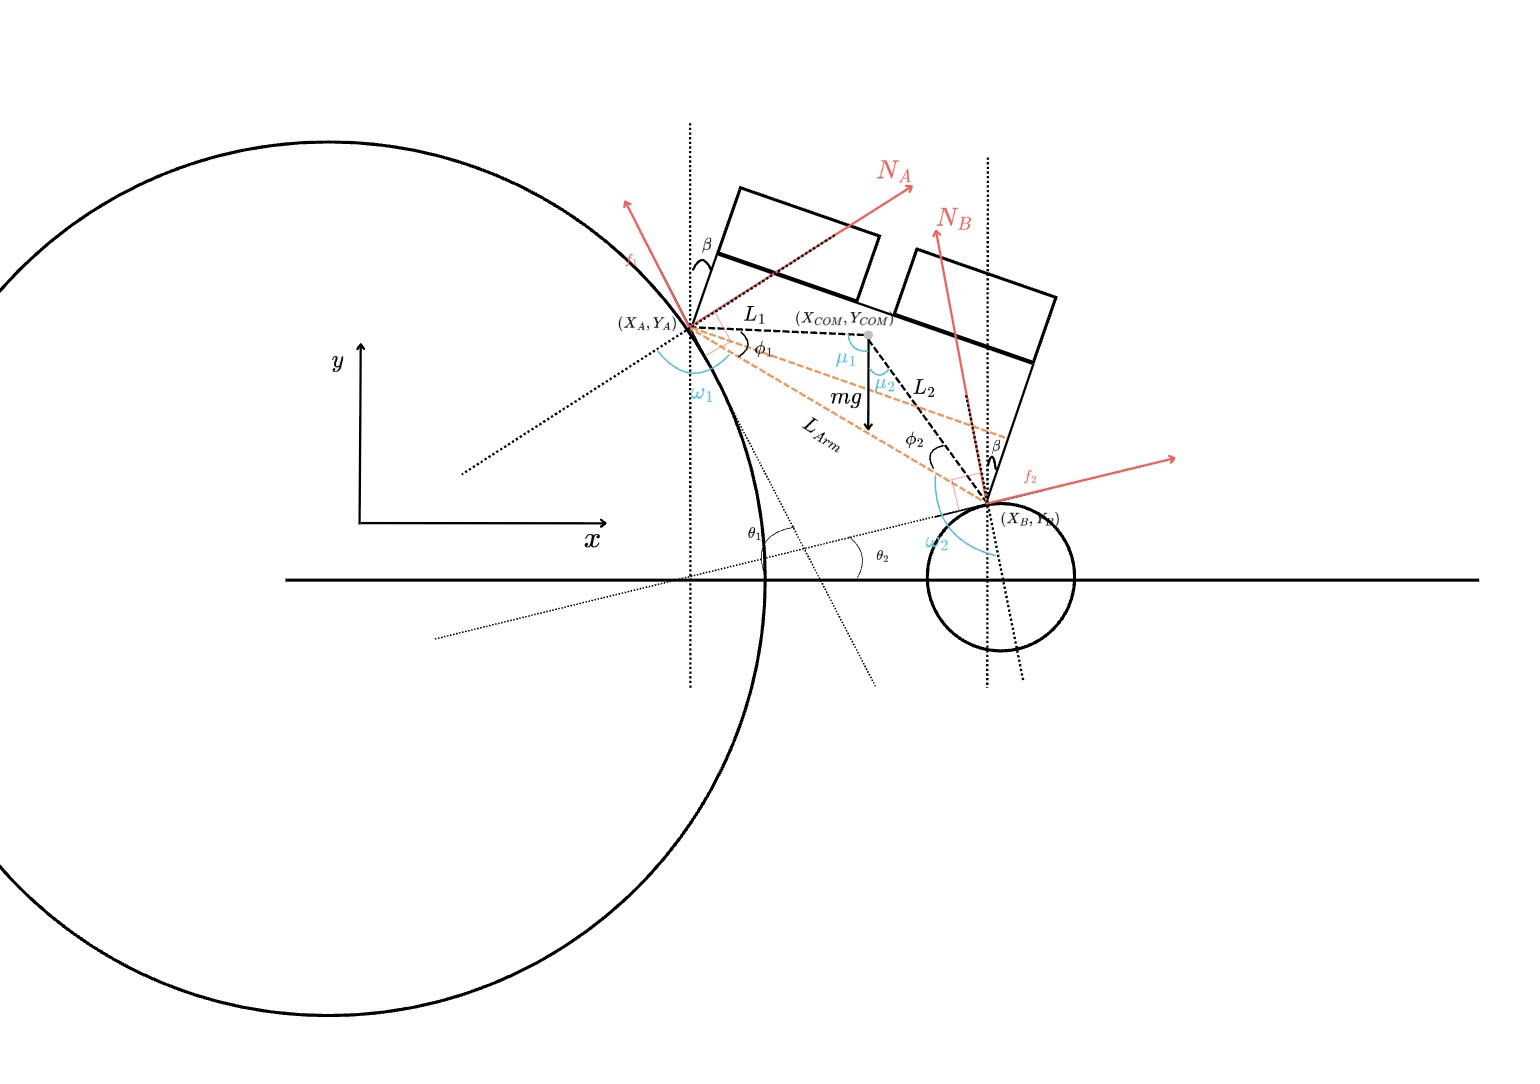
\includegraphics[width=0.8\textwidth]{figs/Generailized expression on Cylinder Terrain.jpg} % replace with your image
\end{center}

With the general expression, we can directly put the same graph within in a cylinder terrian, where
\(\theta_1\) and \(\theta_2\) are esseintially the tangent line with the cylinder. 

\begin{diagram}
    Impossible case under Assumption \ref{ass:leg-ground-contact}
\end{diagram}
\vspace{1ex} % small vertical space
\begin{center}
    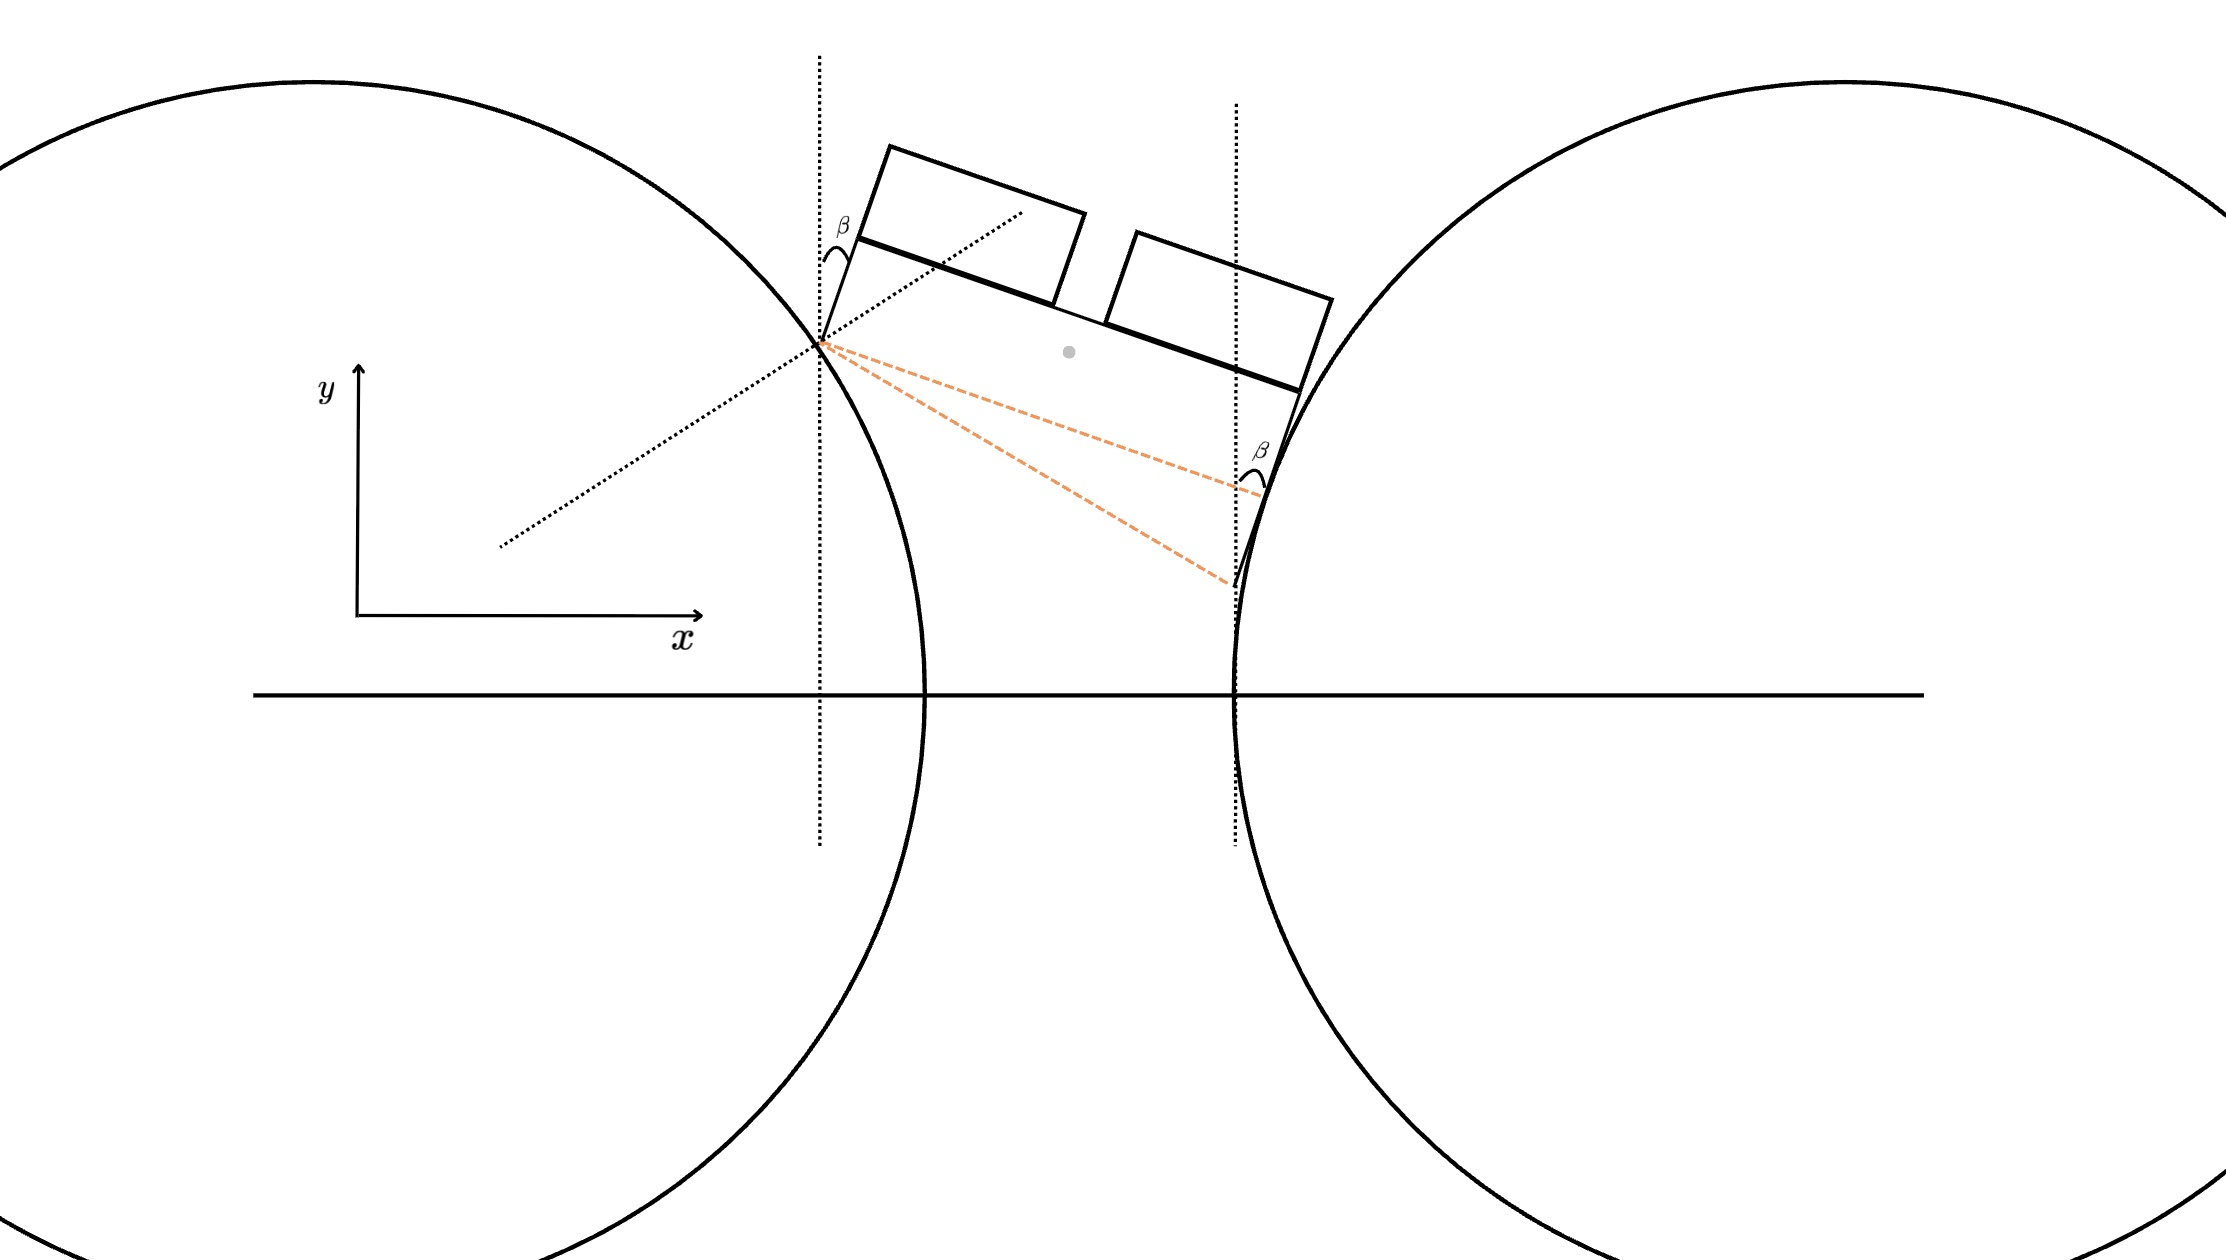
\includegraphics[width=0.8\textwidth]{figs/Impossible case under Assumption.jpg} % replace with your image
\end{center}

However, here, it is impossible that right leg is still contacting the ground due to \(\beta\). In this case, the generalized 
geometric is not applied completely, which requires furthur discuss by changing the assumption \ref{ass:leg-ground-contact}. 

However, this case can also be determined geometrically. Now let's firstly simplify the problem
that all cylinder shape on this terrain has same radius. 

\subsubsection*{Cylinder Terrain when radius are identical}

I made a simple demo for robot geometric shape can be found in this \href{https://www.geogebra.org/classic/vzgc97bq}{GeoGebra link}.
Here A represents the contact point of left leg on the left circle and AB represents of \(L_{Spine}\). The
moving P point represents the right leg extension and AP represents the \(L_{Arm}\).For both folowing cases, 
we form equations as follows in coordinates:

\begin{note}
    In this terrain, what we actually want to consider is given the shape of the cylinder
    (i.e radius and gap), how can we find the \(\theta_1\) and \(\theta_2\).
\end{note}

\begin{diagram}
    When Point P contacts the terrain
\end{diagram}
\vspace{1ex} % small vertical space
\begin{center}
    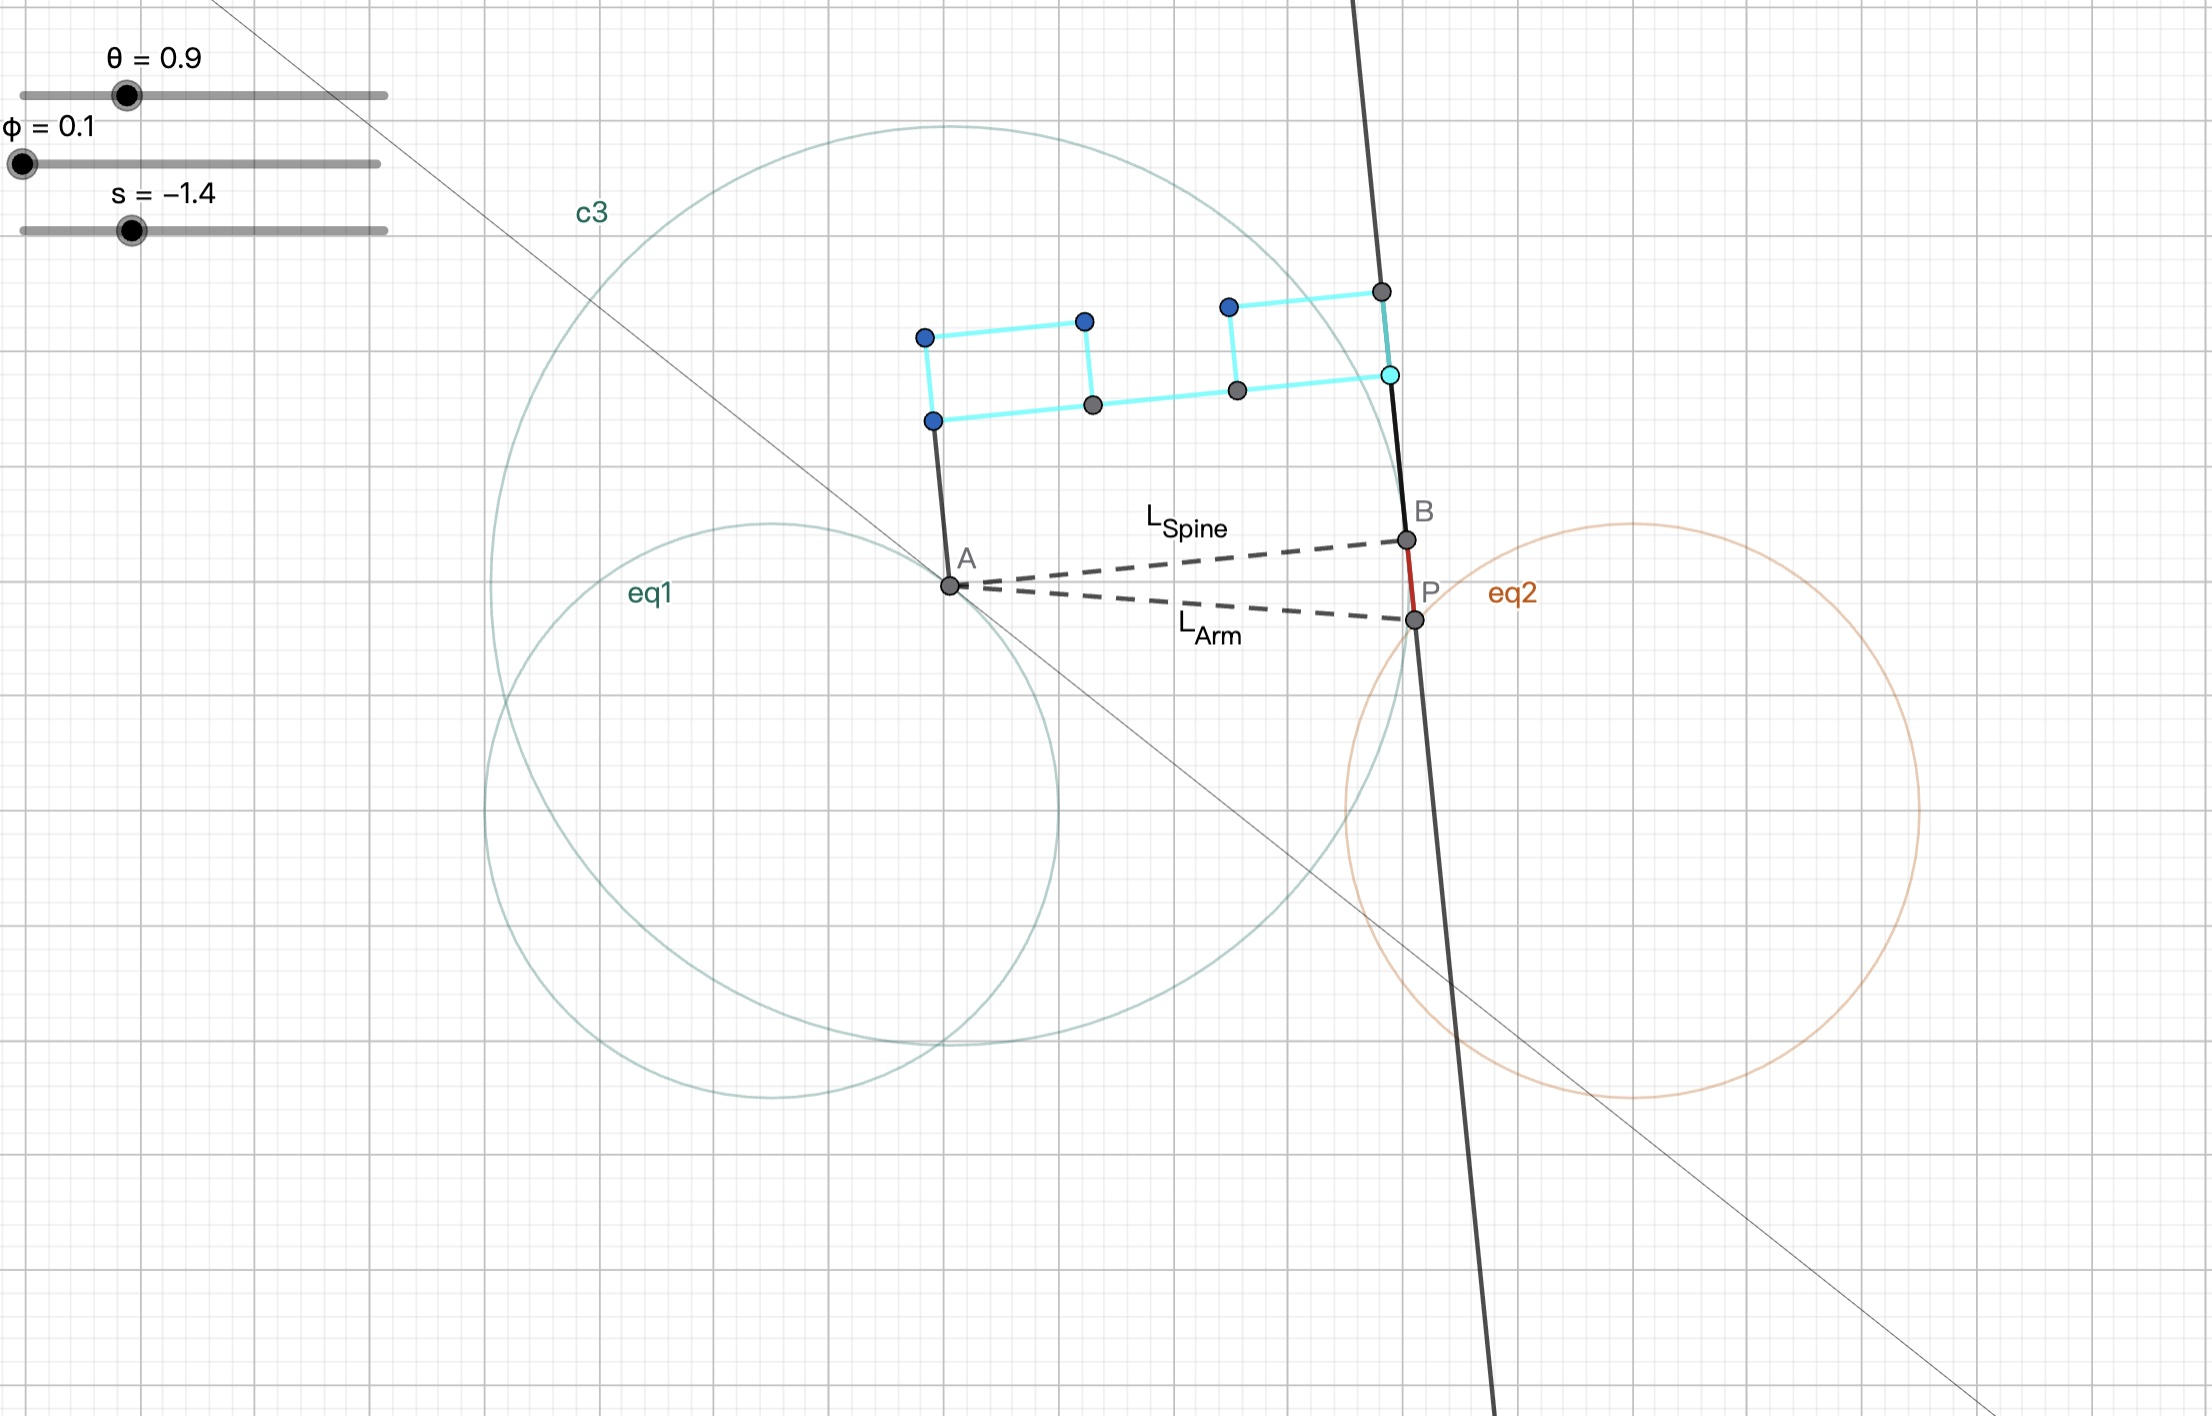
\includegraphics[width=0.5\textwidth]{figs/Cylinder-Case1.jpg} % replace with your image
\end{center}

\begin{diagram}
    When Segment tangents the terrain
\end{diagram}
\vspace{1ex} % small vertical space
\begin{center}
    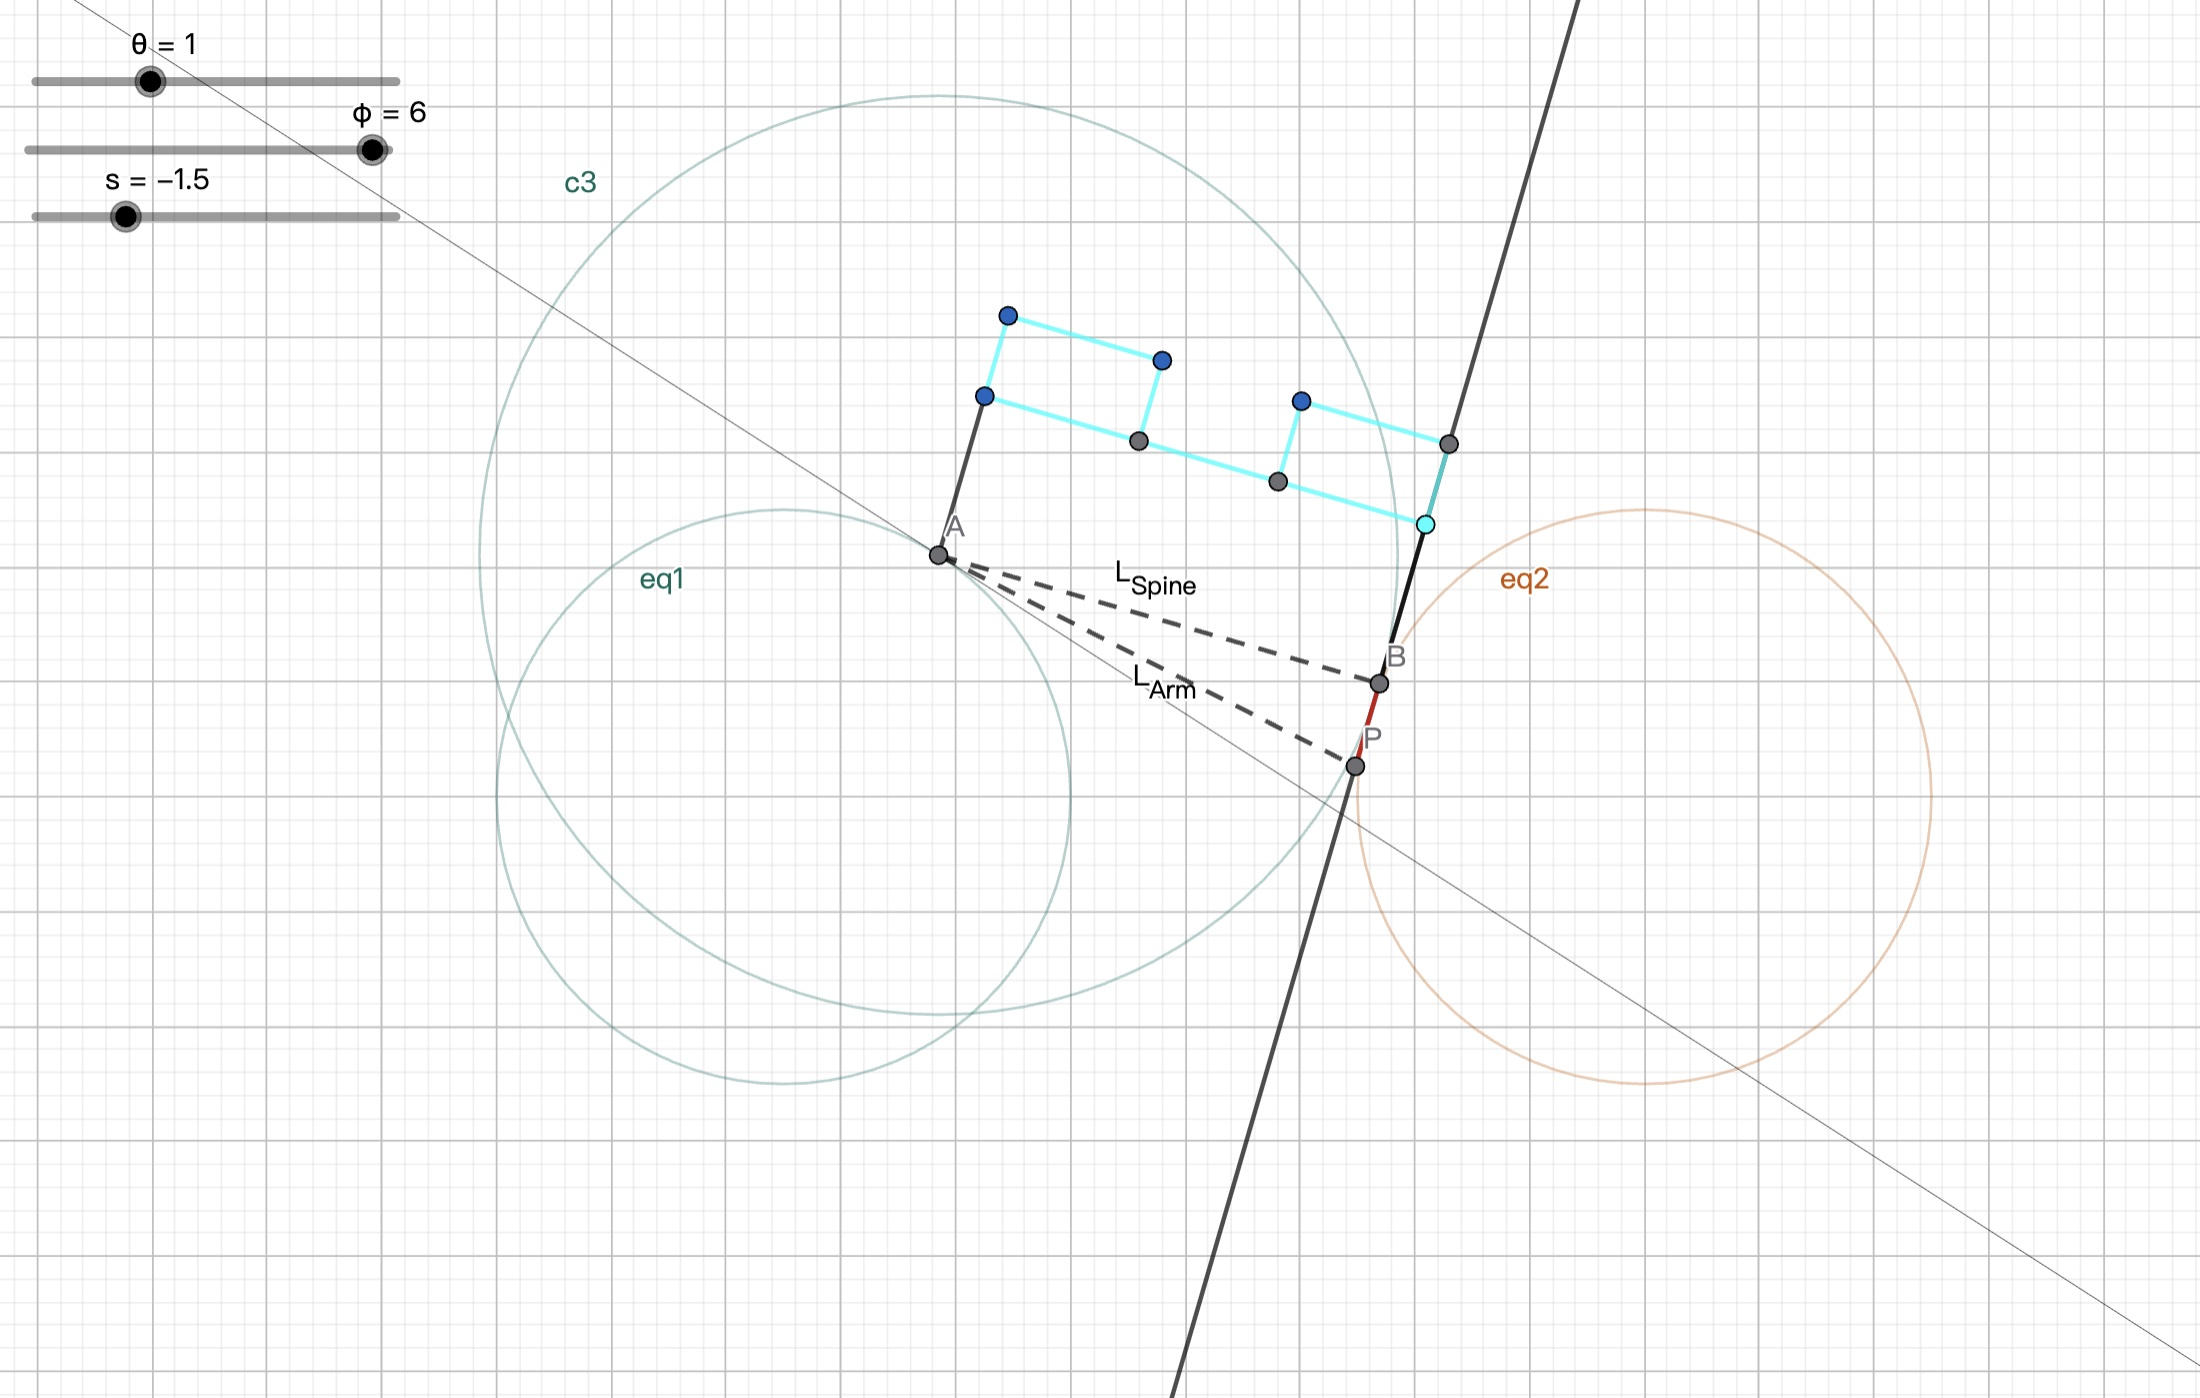
\includegraphics[width=0.5\textwidth]{figs/Cylinder-Case2.jpg} % replace with your image
\end{center}

\noindent\textbf{Obstacle and Terrain Representation}
\begin{align*}
    &\text{Obstacle } c_1&& (x - c_1)^2 + y^2 = r^2 \\\\
    &\text{Obstacle } c_2&& (x - c_2)^2 + y^2 = r^2
\end{align*}

% \noindent\textbf{Flat Terrain Between Obstacles:}
% \begin{equation*}
% \text{TerrainHeight}(x) =
% \begin{cases}
%     h_{\text{obs}}, & x < c_1 - r \\\\
%     h_{\text{gap}}, & c_1 + r \leq x \leq c_2 - r \\\\
%     h_{\text{obs}}, & x > c_2 + r \\\\
%     \text{undefined (wall)}, & \text{otherwise}
% \end{cases}
% \end{equation*}

\vspace{1em}
\noindent\textbf{Control Parameters}
\begin{align*}
    \theta &\in [0, \pi] 
    && \text{\small (defines point $A$ on the upper half of the circle centered at $c_1$)} \\ 
    \varphi &\in [0, 2\pi] 
    && \text{\small (controls the direction of the robot spine extended from point $A$)} \\ 
    s &\in [-L_{\text{leg}}, 0]
    && \text{\small (represents the extension length of the right leg from point $B$)}
\end{align*}

\vspace{1em}
\noindent\textbf{Point Definitions}
\begin{align*}
    A &= (x_0, y_0) = \left(c_1 + r \cos \theta,\ r \sin \theta\right) \\
    B &= (x_1, y_1) = \left(x_0 + L_{\text{spine}} \cos \varphi,\ y_0 + L_{\text{spine}} \sin \varphi\right)
\end{align*}
\vspace{1em}
\noindent\textbf{Body Reachability Circle}
\begin{align*}
    c_A: \quad (x - x_0)^2 + (y - y_0)^2 = L_{Spine}^2
\end{align*}

\vspace{1em}
\noindent\textbf{Direction Vector and Point P}
\begin{align*}
    \vec{t} &= (t_x, t_y) = (-\sin \varphi,\ \cos \varphi) \\
    P &= (x_P, y_P) = (x_1 + s t_x,\ y_1 + s t_y)
\end{align*}

% \vspace{1em}
% \noindent\textbf{Distances}
% \begin{align*}
%     L_{\text{arm}} &= \| \vec{AP} \| = \sqrt{(x_P - x_0)^2 + (y_P - y_0)^2} \\
%     L_{\text{spine}} &= \| \vec{AB} \| = \sqrt{(x_1 - x_0)^2 + (y_1 - y_0)^2}
% \end{align*}

\vspace{1em}
\noindent\textbf{Collision Condition}
% \begin{align*}
%     \text{InsideObstacle2}(P) &= (x_P - c_2)^2 + y_P^2 < r^2 \tag{\text{\small Point $P$ must remain outside Obstacle 2.}}
% \end{align*}
Generally speaking, segment \(\overline{BP}\)  must intersect the boundary of Obstacle 2 exactly once:
\begin{align*}
    \left| \overline{BP} \cap \partial c_2 \right| &= 1 \\
    \overline{BP} \cap c_2^\circ &= \emptyset
\end{align*}

% \noindent\textbf{Collision Condition (Point $(x, y)$ inside obstacle):}
% \begin{align*}
%     \text{InsideObstacle} &= \left[(x - c_1)^2 + y^2 < r^2\right] \lor \left[(x - c_2)^2 + y^2 < r^2\right]
% \end{align*}

\subsubsection*{Case1}
\indent \indent In this case, it is very similar to what we did in the previous sections that we would consider 
pitch angle \(\beta\) in consideration. With that, we can determine triangle with knowning that A and P are 
on \(c_1\) and \(c_2\) and their angle.

\begin{diagram}
    Determine the geometric shape
\end{diagram}
\vspace{1ex} % small vertical space
\begin{center}
    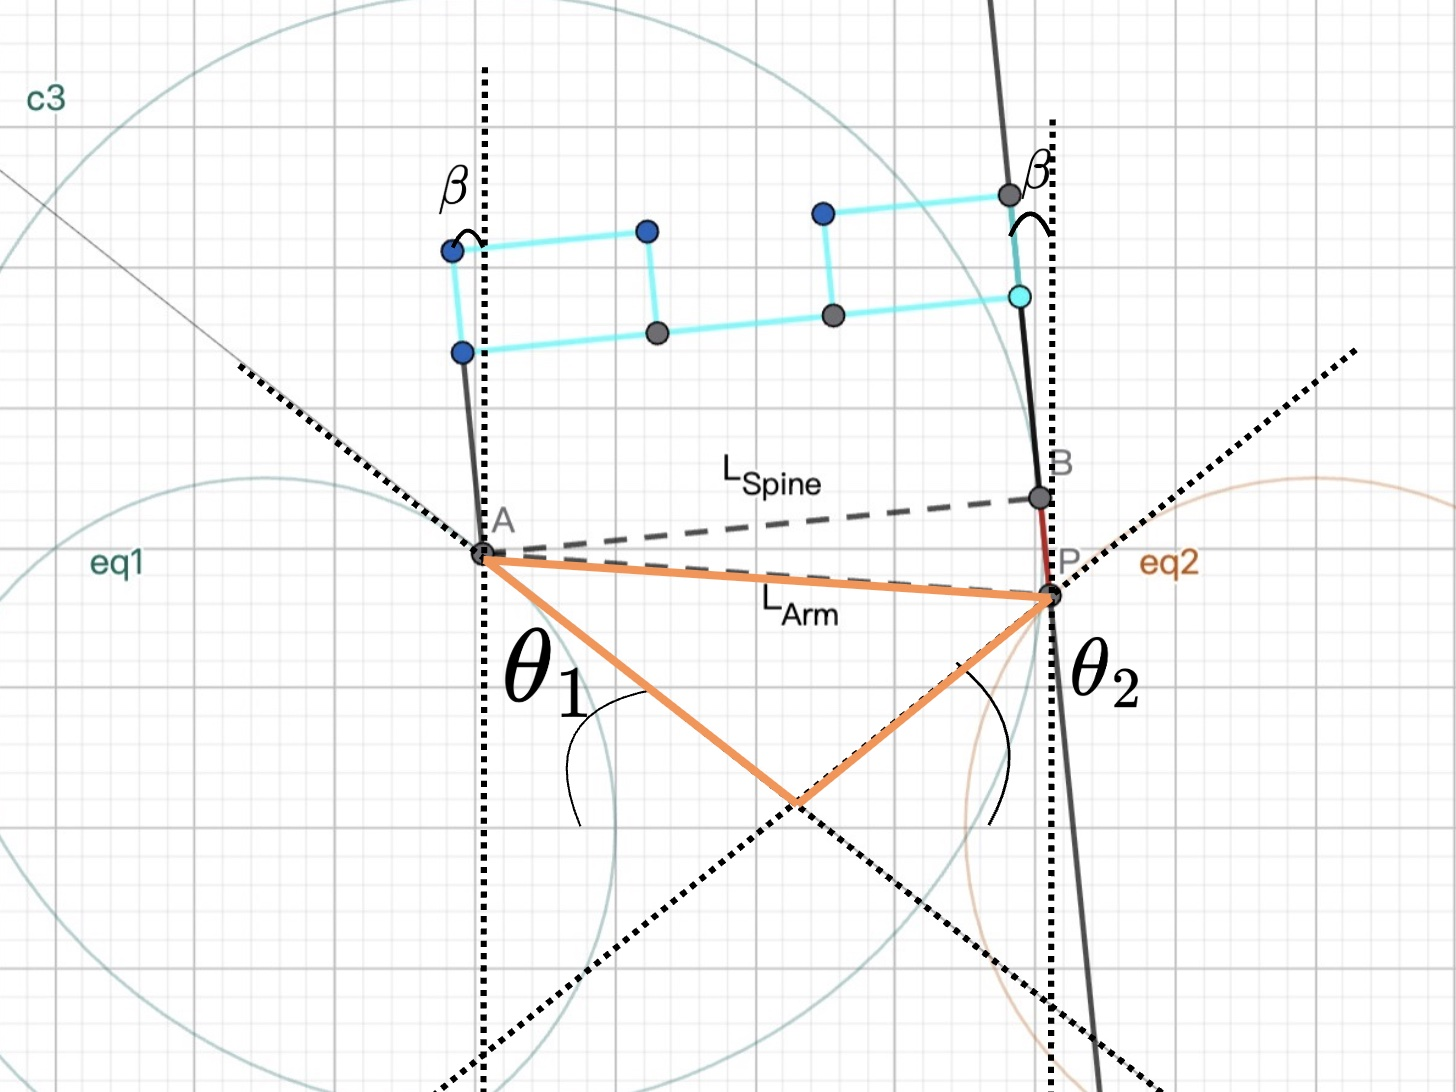
\includegraphics[width=0.5\textwidth]{figs/Cylinder-Case1-Supplementary.jpg} % replace with your image
\end{center}

\begin{itemize}
    \item Two circles $c_1$ and $c_2$ with centers $C_1 = (x_1, y_1)$ and $C_2 = (x_2, y_2)$ respectively, both of radius $r$.
    \item Unknown points $A \in \partial c_1$, $P \in \partial c_2$.
    \item Length $L = \|A - P\|$ is known.
    \item Direction angle of $\vec{AP}$ is known: $\psi \in [0, 2\pi]$ from pitch angle \(\beta\).
\end{itemize}

\begin{note}
    To be more specific, direction angle is derived from both the geometric angle formed by triangle
    ABP and \(\beta\) .
\end{note}

Then the direction vector is:
\[
\vec{d} = \vec{AP} = L(\cos \psi, \sin \psi)
\]

We parameterize:
\begin{align*}
A &= (x_A, y_A) \\
P &= A + \vec{d} = (x_A + L \cos \psi,\ y_A + L \sin \psi)
\end{align*}

Apply the circle constraints:
\begin{align*}
\|A - C_1\|^2 &= r^2 \tag{1} \\
\|P - C_2\|^2 &= r^2 \tag{2}
\end{align*}

Substituting into (2):
\begin{align*}
&\left( x_A + L \cos \psi - x_2 \right)^2 + \left( y_A + L \sin \psi - y_2 \right)^2 = r^2 \tag{2'}
\end{align*}

Now, equations (1) and (2') form a nonlinear system in $x_A, y_A$.

Once $A$ is solved, compute:
\begin{align*}
P &= A + L(\cos \psi, \sin \psi)
\end{align*}

Then, compute the angle between the \textbf{tangent direction} at the contact points and the ground (i.e., the horizontal x-axis). The tangent direction at a point on a circle is perpendicular to the radial vector from the circle's center to that point.

Let the centers of the circles be $C_1 = (x_1, y_1)$ and $C_2 = (x_2, y_2)$, and the contact points be $A = (x_A, y_A)$ and $P = (x_P, y_P)$. The radial vectors are:

\[
\vec{n}_1 = A - C_1 = (x_A - x_1,\ y_A - y_1), \quad
\vec{n}_2 = P - C_2 = (x_P - x_2,\ y_P - y_2)
\]

The corresponding tangent vectors (obtained by rotating the radial vectors 90° clockwise) are:

\[
\vec{t}_1 = (-(y_A - y_1),\ x_A - x_1), \quad
\vec{t}_2 = (-(y_P - y_2),\ x_P - x_2)
\]

The angles between the tangent vectors at the contact points and the ground (horizontal axis) are given by:

\[
\theta_1 = \mathrm{mod}\left( \arctan2(t_{1,y},\ t_{1,x}),\ 2\pi \right)
\]
\[
\theta_2 = \mathrm{mod}\left( \arctan2(t_{2,y},\ t_{2,x}),\ 2\pi \right)
\]

These angles represent the \textbf{oriented direction} of the tangents relative to the ground, measured counterclockwise from the positive \(x\)-axis and wrapped into the interval \([0,\ 2\pi)\).



\subsubsection*{Case2}

\indent \indent For case 2, we can express that tangent line for robot body reachability circle
at point B also must tanget with \(c_2\). Therefore we can formulate:
\begin{align*}
    &\text{Let } \vec{n} := B - A \\
    &\text{Define a line } \ell \text{ such that:} \\
    &\quad B \in \ell,\quad \vec{d}_\ell \cdot \vec{n} = 0 \quad \text{i.e., }\ell \text{ is tangent to } c_A \text{ at } B \\
    &\quad \exists\ P' \in \ell \cap \partial c_2,\quad \vec{d}_\ell \cdot (P' - C_2) = 0 \quad \text{i.e., } \ell \text{ is tangent to } c_2 \text{ at } P'\\
    &\quad \abs{BP'} \leq \abs{BP}
\end{align*}

\begin{note}
    For Case2, the pitch angle \(\beta\) does not matter and we can still find at most one solution.
\end{note}

Let $\vec{d}_\ell$ be the direction vector of $\ell$, defined by:
\begin{align*}
    \vec{d}_\ell &= (-n_y,\ n_x) \quad \text{(perpendicular to } \vec{n} = B - A\text{)}
\end{align*}

Then, the parametric equation of $\ell$ is:
\begin{align*}
    \ell(\lambda) &= B + \lambda \vec{d}_\ell
\end{align*}

To ensure tangency with $c_2$, we require:
\begin{align*}
    \|\ell(\lambda) - C_2\|^2 &= r^2
\end{align*}
which leads to a quadratic in $\lambda$:
\begin{align*}
    \|B + \lambda \vec{d}_\ell - C_2\|^2 &= r^2
\end{align*}

Solving this yields candidate point(s) $P' = B + \lambda^* \vec{d}_\ell$.
Select the point that satisfies:
\begin{align*}
    \|BP'\| &\leq \|BP\|
\end{align*}

Finally, the center $A$ of $c_A$ is obtained by inverting $\vec{n}$:
\begin{align*}
    \vec{n}_{\text{unit}} &= \frac{\vec{n}}{\|\vec{n}\|} \\
    A &= B - R \cdot \vec{n}_{\text{unit}}
\end{align*}

This determines $A$ and $P'$ geometrically under the tangency constraints.

\newpage
\section{From d'Alembert principle to Dynamics}
The d'Alembert principle provides a natural bridge from statics to dynamics. 
% It states that the dynamics of a mechanical system can be described as a 
% generalized static equilibrium, once the inertial forces are included. 
% For a system of particles, the principle is written as:

\begin{theorem}\label{thm:ld'Alembert}
    \[
    \sum_i \left( \mathbf{F}_i - m_i \mathbf{a}_i \right) \cdot \delta \mathbf{r}_i = 0
    \]
\end{theorem}

where $\mathbf{F}_i$ is the applied force on the $i$-th particle, $m_i \mathbf{a}_i$ is its inertial force, and $\delta \mathbf{r}_i$ denotes any virtual displacement compatible with the system's constraints.

Let the position of the robot's center of mass be denoted by \( \mathbf{r}_G^\mathcal{I} \in \mathbb{R}^2 \). And two leg contact position
as \( \mathbf{p}_A^\mathcal{I} \)  and \( \mathbf{p}_B^\mathcal{I} \).

\subsection{Holonomic constraints:}

Using the identity \( \sin(\arctan(x)) = \frac{x}{\sqrt{1 + x^2}} \), the geometric constraint imposed by the spine length can be rewritten as:

\[
L_\text{Arm} = \left\| \mathbf{p}_B^\mathcal{I} - \mathbf{p}_A^\mathcal{I} \right\| =
\frac{L_\text{Spine}^2}{\sqrt{L_\text{Spine}^2 + \left(L_{\text{Leg}2} - L_{\text{Leg}1}\right)^2}}
\]

The terrain contact constraints are then written as:

\[
f_A := p_{A,y}^\mathcal{I} - h(p_{A,x}^\mathcal{I}) = 0, \quad
f_B := p_{B,y}^\mathcal{I} - h(p_{B,x}^\mathcal{I}) = 0
\]

In general, the center of mass can be written as a function of the two foot positions \( \mathbf{p}_A^\mathcal{I} \) and \( \mathbf{p}_B^\mathcal{I} \), depending on the mass distribution and geometry:

\[
\mathbf{r}_G^\mathcal{I} = \mathbf{f}_G\left( \mathbf{p}_A^\mathcal{I}, \mathbf{p}_B^\mathcal{I} , \beta \right)
\]
where \( \beta \) is the pitch angle of the spine, measured from horizontal and it can be derived through
\(\mathbf{f}_{\beta}(\mathbf{p}_A^\mathcal{I},\mathbf{p}_B^\mathcal{I},L_\text{Spine},L_{\text{Leg}1},L_{\text{Leg}2})\) 
by geometric constrains following:
\begin{enumerate}
    \item $\|\mathbf{q}_1 - \mathbf{p}_A\| = L_\text{Leg1}$
    \item $\|\mathbf{q}_2 - \mathbf{p}_B\| = L_\text{Leg2}$
    \item $\|\mathbf{q}_2 - \mathbf{q}_1\| = L_\text{Spine}$
    \item Directional constraint: 
    \[
        \mathbf{q}_1 - \mathbf{p}_A \parallel \mathbf{q}_2 - \mathbf{p}_B 
        \Rightarrow 
        (\mathbf{q}_1 - \mathbf{p}_A) = \lambda (\mathbf{q}_2 - \mathbf{p}_B)
    \]
\end{enumerate}
Therefore, we get:
\begin{align*}
& (x_1 - x_A)^2 + (y_1 - y_A)^2 = L_{\text{Leg}1}^2 \\[0.5em]
& (x_2 - x_B)^2 + (y_2 - y_B)^2 = L_{\text{Leg}2}^2 \\[0.5em]
& (x_2 - x_1)^2 + (y_2 - y_1)^2 = L_{\text{Spine}}^2 \\[0.5em]
& (x_1 - x_A)(y_2 - y_B) - (y_1 - y_A)(x_2 - x_B) = 0
\end{align*}

And therefore, we can get the solution of \(x_1, x_2, y_1, y_2\) through numerical method. 
And then, we can find the \(\beta\) by: 
\[
\beta = \operatorname{atan2}\!\bigl(y_1 - y_A,\; x_1 - x_A\bigr) \\[6pt]
\]  

Furthure more, we can even determine the \textbf{CoM} by: 
\[
\mathbf{r}_G^\mathcal{I} =
\begin{bmatrix}
x_m \\
y_m
\end{bmatrix}
+
d \begin{bmatrix}
\cos\beta \\
\sin\beta
\end{bmatrix},
\quad
\text{where} \quad
\begin{bmatrix}
x_m \\
y_m
\end{bmatrix}
=
\frac{1}{2}
\begin{bmatrix}
x_1 + x_2 \\
y_1 + y_2
\end{bmatrix},
\text{and } d 
\text{ is offset} 
\]

\subsection{Non-Holonomic constraints:}
\indent \indent There are none.

\vspace{10pt}
Therefore, the total \textbf{DoF} is \(3N-5 =1\). This indicates we can desribe the whole system through one generalized
coordinate. And we can choose \(x_{A}^{\mathcal{I}}\) for simplicity. We can describe as \( q := x_A^\mathcal{I} \). All other quantities can be written as functions of \( q \) due to the holonomic constraints.
\[
\mathbf{p^\mathcal{I}}_A(q) =
\begin{bmatrix}
q \\
h(q)
\end{bmatrix}, \quad
\mathbf{p^\mathcal{I}}_B(q) =
\begin{bmatrix}
\mathbf{f}_B(q) \\
h(\mathbf{f}_B(q))
\end{bmatrix}, \quad
\mathbf{r}_G^\mathcal{I} =
\begin{bmatrix}
\mathbf{f}_{Gx}(q) \\
\mathbf{f}_{Gy}(q)
\end{bmatrix}
\]

Then, the velocity and acceleration of the \textbf{CoM} can be expressed as:
\[
\dot{\mathbf{r}}_G = \frac{d \mathbf{f}_G}{dq} \cdot \dot{q}, \quad
\ddot{\mathbf{r}}_G = \frac{d \mathbf{f}_G}{dq} \cdot \ddot{q} + \frac{d^2 \mathbf{f}_G}{dq^2} \cdot \dot{q}^2
\]

Therefore, through d'Alembert principle, we write:
\[
\left(\mathbf{f}_A + \mathbf{f}_B 
+ \mathbf{F}_g 
- m\ddot{\mathbf{r}}_G \right) 
\cdot \delta \mathbf{r}_G = 0
\]

\subsection{Sinusoidal Terrain}
\indent \indent Lets start with the sinusoidal terrain where the terrain is easy to express with one function:

\[
h(x^\mathcal{I}) = A \cdot \sin\left( \frac{2\pi}{T} x^\mathcal{I} + \phi \right) + B
\]

We can set \(B\) as \(\frac{A}{2}\) and \(\theta\) as 0 and gives us: 

\[
h(x^\mathcal{I}) = A \cdot \sin\left( \frac{2\pi}{T} x^\mathcal{I} \right) + \frac{A}{2}
\]

Therefore, we can express our three key points explicitly as:

\[
\footnotesize
\setlength{\arraycolsep}{6pt}   % space between columns
\renewcommand{\arraystretch}{1.05}% vertical row spacing
\begin{array}{@{}l@{\qquad}l@{}}
%%%%%%%%%%%%%%%%%%%%%%%%%%%%%%%%%%%%%%%%%%%%%%%%%%%%%%%%%%%%
\mathbf{p}_A^\mathcal{I}(q)=
\begin{bmatrix}
q\\
A\sin\!\bigl(\tfrac{2\pi}{T}q\bigr)+\tfrac{A}{2}
\end{bmatrix}
&
\text{directly defined by } q
\\[.8em]
\noalign{\hrule height 0.35pt}
%%%%%%%%%%%%%%%%%%%%%%%%%%%%%%%%%%%%%%%%%%%%%%%%%%%%%%%%%%%%
\mathbf{p}_B^\mathcal{I}(q)=
\begin{bmatrix}
x_B(q)\\
A\sin\!\bigl(\tfrac{2\pi}{T}x_B(q)\bigr)+\tfrac{A}{2}
\end{bmatrix}
&
\begin{aligned}
x_B(q)\ \text{solves:}\quad
(x_B-q)^2
&+\Bigl[A\sin\!\bigl(\tfrac{2\pi}{T}x_B\bigr)
      -A\sin\!\bigl(\tfrac{2\pi}{T}q\bigr)\Bigr]^2
      =L_{\text{Arm}}^{\,2}
\end{aligned}
\\[.8em]
\noalign{\hrule height 0.35pt}
%%%%%%%%%%%%%%%%%%%%%%%%%%%%%%%%%%%%%%%%%%%%%%%%%%%%%%%%%%%%
\mathbf{r}_G^\mathcal{I}(q)=
\begin{bmatrix}
x_m\\
y_m
\end{bmatrix}
+
d\!
\begin{bmatrix}
\cos\beta\\
\sin\beta
\end{bmatrix}
&
\begin{aligned}
x_m &=\tfrac12(x_1+x_2),\quad
y_m=\tfrac12(y_1+y_2)\\[2pt]
\beta &=\operatorname{atan2}(y_1-y_A,\;x_1-x_A)\\[4pt]
x_1, x_2, y_1, y_2\ \text{solves:}\quad
(x_1-x_A)^2+(y_1-y_A)^2 &=L_{\text{Leg}1}^2\\
(x_2-x_B)^2+(y_2-y_B)^2 &=L_{\text{Leg}2}^2\\
(x_2-x_1)^2+(y_2-y_1)^2 &=L_{\text{Spine}}^2\\
(x_1-x_A)(y_2-y_B) -\,(y_1-y_A)(x_2-x_B)&=0
\end{aligned}
\end{array}
\]

Therefore, we can now expand out the equation for virtual work as follows:

\[
\left(
\mathbf{f}_A \cdot \frac{d\mathbf{p}_A}{dq}
+ \mathbf{f}_B \cdot \frac{d\mathbf{p}_B}{dq}
+ \mathbf{F}_g \cdot \frac{d\mathbf{r}_G}{dq}
- m \ddot{\mathbf{r}}_G \cdot \frac{d\mathbf{r}_G}{dq}
\right)
\delta q = 0
\]

\[
\begin{aligned}
\mathbf{f}_A &= 
\lambda_N^A \, \hat{\mathbf{n}}_A +
\lambda_f^A \, \hat{\mathbf{t}}_A +
\lambda_{\parallel}^A \, \hat{\mathbf{e}}_\beta +
\lambda_{\perp}^A \, \hat{\mathbf{e}}_\beta^\perp \\[0.5em]
\mathbf{f}_B &= 
\lambda_N^B \, \hat{\mathbf{n}}_B +
\lambda_f^B \, \hat{\mathbf{t}}_B +
\lambda_{\parallel}^B \, \hat{\mathbf{e}}_\beta +
\lambda_{\perp}^B \, \hat{\mathbf{e}}_\beta^\perp
\end{aligned}
\]

where we can expand out as:
\[
\begin{aligned}
&\Big(
\underbrace{
\lambda_N^A \, \hat{\mathbf{n}}_A \cdot \frac{d\mathbf{p}_A}{dq}
+ \lambda_f^A \, \hat{\mathbf{t}}_A \cdot \frac{d\mathbf{p}_A}{dq}
+ \lambda_{\parallel}^A \, \hat{\mathbf{e}}_\beta \cdot \frac{d\mathbf{p}_A}{dq}
+ \lambda_{\perp}^A \, \hat{\mathbf{e}}_\beta^\perp \cdot \frac{d\mathbf{p}_A}{dq}
}_{\mathbf{f}_A \cdot \frac{d\mathbf{p}_A}{dq}} \\[0.8em]
&\quad
+ \underbrace{
\lambda_N^B \, \hat{\mathbf{n}}_B \cdot \frac{d\mathbf{p}_B}{dq}
+ \lambda_f^B \, \hat{\mathbf{t}}_B \cdot \frac{d\mathbf{p}_B}{dq}
+ \lambda_{\parallel}^B \, \hat{\mathbf{e}}_\beta \cdot \frac{d\mathbf{p}_B}{dq}
+ \lambda_{\perp}^B \, \hat{\mathbf{e}}_\beta^\perp \cdot \frac{d\mathbf{p}_B}{dq}
}_{\mathbf{f}_B \cdot \frac{d\mathbf{p}_B}{dq}} \\[0.8em]
&\quad
+ \mathbf{F}_g \cdot \frac{d\mathbf{r}_G}{dq}
- m \ddot{\mathbf{r}}_G \cdot \frac{d\mathbf{r}_G}{dq}
\Big) \delta q = 0
\end{aligned}
\]

\begin{itemize}
  \item[1.] \( \lambda_N^A \, \hat{\mathbf{n}}_A \cdot \frac{d\mathbf{p}_A}{dq} = 0 \)  
        (Normal force is perpendicular to virtual displacement: does no work)

  \item[2.] \( \lambda_f^A \, \hat{\mathbf{t}}_A \cdot \frac{d\mathbf{p}_A}{dq}
  = \lambda_f^A \cdot \left\| \frac{d\mathbf{p}_A}{dq} \right\| \),  
  because \( \hat{\mathbf{t}}_A \parallel \frac{d\mathbf{p}_A}{dq} \)

  \item[3.] \( \left( \lambda_{\parallel}^A \cdot \frac{d\mathbf{p}_A}{dq}
    + \lambda_{\parallel}^B \cdot \frac{d\mathbf{p}_B}{dq} \right)
    \cdot \hat{\mathbf{e}}_\beta \)  
    (Combined contribution of spine-direction forces at A and B)

  \item[4.] \( \left( \lambda_{\perp}^A \cdot \frac{d\mathbf{p}_A}{dq}
    + \lambda_{\perp}^B \cdot \frac{d\mathbf{p}_B}{dq} \right)
    \cdot \hat{\mathbf{e}}_\beta^\perp \)  
    (Combined contribution of perpendicular forces along the direction orthogonal to the spine)

    \item[5.]  % ——B-point friction term
    \[
    \boxed{
    \hat{\mathbf{t}}_B =
    \frac{1}{\sqrt{1 + \left( h'(x_B) \right)^2}}
    \begin{bmatrix}
    1 \\
    h'(x_B)
    \end{bmatrix}
    }, \qquad
    \boxed{
    \hat{\mathbf{n}}_B =
    \frac{1}{\sqrt{1 + \left( h'(x_B) \right)^2}}
    \begin{bmatrix}
    - h'(x_B) \\
    1
    \end{bmatrix}
    }.
    \]
\end{itemize}

\newpage
\subsection{Zig-Zag Terrain}
The zig-zag terrain is defined by a periodic piecewise function \( y = h(x^\mathcal{I}) \), with period \( T = 2r + d \) and height \( h = r \tan\theta \). For each point \( x^\mathcal{I} \in \mathbb{R} \), define \( x_k = x^\mathcal{I} \bmod T \). Then:

\[
h(x^\mathcal{I}) =
\begin{cases}
\tan\theta \cdot x_k, & x_k \in [0, r] \\
\tan\theta \cdot (2r - x_k), & x_k \in [r, 2r] \\
0, & x_k \in [2r, 2r + d]
\end{cases}
\]

Here, in order to make the terrain differentiable at any point, we can use fourier series to approximate the terrain like:

\[
h(x^\mathcal{I}) = \frac{8 r \tan\theta}{\pi^2} \sum_{n=1,3,5,\dots}^{N} \frac{1}{n^2} \cos\left( \frac{2\pi n x}{2r + d} \right)
\]

% \subsection*{Cylinder Terrain}
% Lets firstly parameterize our target terrain as:
% \[
% y = 
% \begin{cases}
% 0, & x_0 + (a + 2r)k \leq x \leq x_0 + (a + 2r)k + a \\
% \sqrt{r^2 - (x - (a + r))^2}, & x_0 + (a + 2r)k + a \leq x \leq x_0 + (a + 2r)k + a + 2r
% \end{cases}
% \]

% \noindent
% where \( a \) is the gap distance between curved segments, and \( x_0 \) is the initial offset.

\end{document}
